\subsection{XboxControllerklassen} \label{sec:xboxcontroller_impl}

XboxController er en klasse der har til formål er at give PC softwaren mulighed for at læse Xbox controllerens tilstand. Klassens primære funktion er altså at agere API for PC softwaren.
Herunder vil koden blive forklaret i detaljer.


\paragraph{XboxController Constructor} er klassens constructor. Den tager imodet argument til at bestemme controllerens ID. Koden er vist i Listing \ref{lst:xboxcontroller_con}.

\lstinputlisting[linerange=XboxController::XboxController1-XboxController::XboxController2, label=lst:xboxcontroller_con, caption=\texttt{XboxController} Constructor.]{../../src/pc/XboxController/xboxcontroller.h}


\paragraph{getNumber} er en funktion der returnere det pågældende objects ID. Denne funktion bruges ikke i hovedprogrammet, men udnyttes til testing. Koden er vist i Listing \ref{lst:getnumber}.

\lstinputlisting[linerange=XboxController::getNumber1-XboxController::getNumber2, label=lst:getnumber, caption=Funktionen \texttt{getNumber}.]{../../src/pc/XboxController/xboxcontroller.h}


\paragraph{getState} er en funktion der sørger for først at fylde \texttt{XINPUT\_STATE} structen \texttt{\_controllerState}, med nuller. Herefter indskrives Xbox Controllerens nuværende tilstand ind i denne struct der har alle plads til alt information om en Xbox Controllers forskellige dele. Til sidst returneres \texttt{\_controllerState}. Koden kan ses på Listing \ref{lst:getstate}.

\lstinputlisting[linerange=XboxController::getState1-XboxController::getState2, label=lst:getstate, caption=Funktionen \texttt{getState}.]{../../src/pc/XboxController/xboxcontroller.h}

\clearpage

\paragraph{connect} er en funktion til at oprette forbindelse mellem API og controller enheden. Den fungerer på samme måde som \texttt{getState} men returnerer ikke controllerens tilstand, men derimod om hvorvidt der er forindelse mellem controller enheden og klassen. Koden kan ses på Listing \ref{lst:connect}.

\lstinputlisting[linerange=XboxController::connect1-XboxController::connect2, label=lst:connect, caption=Funktionen \texttt{connect}.]{../../src/pc/XboxController/xboxcontroller.h}


\paragraph{vibrate} er en funktion til at håndterer vibraterne i controlleren. Der er hhv. en venstre og en højre motor i en Xbox Controller som begge kan tage imod en værdi mellem 0 og 255, hvor 0 stopper motoren og 255 sætter motoren i maks hastighed. Denne funktion bliver ikke udnyttet i selve systemet, men er brugt til at kunne teste hvorvidt der er skabt en forbindelse der også giver mulighed for at skrive funktionalitet ud til controlleren.  Koden kan ses på Listing \ref{lst:vibrate}.

\lstinputlisting[linerange=XboxController::vibrate1-XboxController::vibrate2, label=lst:vibrate, caption=Funktionen \texttt{vibrate}.]{../../src/pc/XboxController/xboxcontroller.h}

\clearpage

\paragraph{getCtrData} er en funktion der er lavet for at simplificere PC softwarens metodekald. Funktionen sender de fire ønskede informationer om controllerens tilstand, hhv. Left Stick, Right Trigger, Left Trigger og X-knappens tilstande. Til dette udnyttes call-by-reference, dvs. at ved funktionskaldet tager funktionen imod fire referencer der ønskes at skreven direkte til. Ud over dette sørger funktionen for at caste alle værdier til den ønskede værdi ifølge protokolen under afsnit \ref{tbl:prt_controller_byte} \nameref{tbl:prt_controller_byte} på side \pageref{tbl:prt_controller_byte}. Koden for funktionene er vist i Listing \ref{lst:getctrdata}.

\lstinputlisting[linerange=XboxController::getCtrData1-XboxController::getCtrData2, label=lst:getctrdata, caption=Funktionen \texttt{getCtrData}.]{../../src/pc/XboxController/xboxcontroller.h}

\subsubsection{Test af XboxControllerklassen}
Denne klasse er testet med et testprogram, der udskriver de hentede tilstande fra controlleren i et konsolvindue. Testresultatet kan ses på figur \ref{fig:xboxcontroller_test}.

\begin{figure}[h!]
\centering
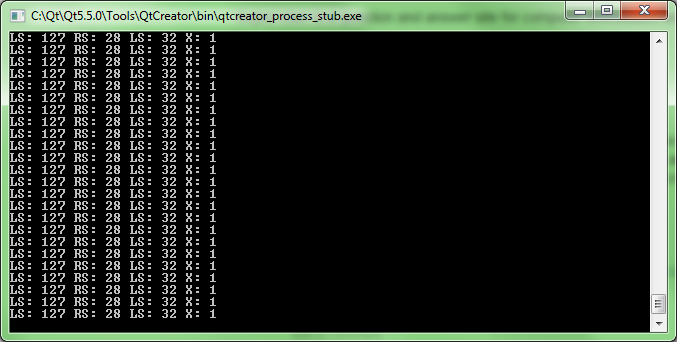
\includegraphics[width=\textwidth* 3/4]{../fig/billeder/xboxcontroller_test.png}
\caption{Xboxcontroller Testresultat}
\label{fig:xboxcontroller_test}
\end{figure}

\clearpage